% Options for packages loaded elsewhere
\PassOptionsToPackage{unicode}{hyperref}
\PassOptionsToPackage{hyphens}{url}
%
\documentclass[twoside]{report}
\usepackage{lmodern}
\usepackage{amssymb,amsmath}
\usepackage{ifxetex,ifluatex}
\ifnum 0\ifxetex 1\fi\ifluatex 1\fi=0 % if pdftex
  \usepackage[T1]{fontenc}
  \usepackage[utf8]{inputenc}
  \usepackage{textcomp} % provide euro and other symbols
\else % if luatex or xetex
  \usepackage{unicode-math}
  \defaultfontfeatures{Scale=MatchLowercase}
  \defaultfontfeatures[\rmfamily]{Ligatures=TeX,Scale=1}
\fi
% Use upquote if available, for straight quotes in verbatim environments
\IfFileExists{upquote.sty}{\usepackage{upquote}}{}
\IfFileExists{microtype.sty}{% use microtype if available
  \usepackage[]{microtype}
  \UseMicrotypeSet[protrusion]{basicmath} % disable protrusion for tt fonts
}{}

\usepackage{tocloft}
\renewcommand{\cftsecfont}{\bfseries}
\renewcommand{\cftsubsecfont}{\itshape}
\renewcommand{\cftsubsubsecfont}{\small}
\renewcommand{\cftparafont}{\footnotesize}
\renewcommand{\cftsubparafont}{\scriptsize}
\renewcommand{\cftdotsep}{1}
%\renewcommand{\cftZtitlefont}{\Large}

\usepackage[lf]{Baskervaldx}
\usepackage[vvarbb]{newtxmath}
\usepackage[cal=boondoxo]{mathalfa}
\makeatletter
\@ifundefined{KOMAClassName}{% if non-KOMA class
  \IfFileExists{parskip.sty}{%
    \usepackage{parskip}
  }{% else
    \setlength{\parindent}{0pt}
    \setlength{\parskip}{6pt plus 2pt minus 1pt}}
}{% if KOMA class
  \KOMAoptions{parskip=half}}
\makeatother
\usepackage{xcolor}

\usepackage{longtable,booktabs}
% Correct order of tables after \paragraph or \subparagraph
\usepackage{etoolbox}
\makeatletter
\patchcmd\longtable{\par}{\if@noskipsec\mbox{}\fi\par}{}{}
\makeatother
% Allow footnotes in longtable head/foot
\IfFileExists{footnotehyper.sty}{\usepackage{footnotehyper}}{\usepackage{footnote}}
\makesavenoteenv{longtable}
\usepackage{graphicx,grffile}
\graphicspath{ {./images/} }
\makeatletter
\def\maxwidth{\ifdim\Gin@nat@width>\linewidth\linewidth\else\Gin@nat@width\fi}
\def\maxheight{\ifdim\Gin@nat@height>\textheight\textheight\else\Gin@nat@height\fi}
\makeatother
% Scale images if necessary, so that they will not overflow the page
% margins by default, and it is still possible to overwrite the defaults
% using explicit options in \includegraphics[width, height, ...]{}
\setkeys{Gin}{width=\maxwidth,height=\maxheight,keepaspectratio}
% Set default figure placement to htbp
\makeatletter
\def\fps@figure{htbp}
\makeatother
\setlength{\emergencystretch}{3em} % prevent overfull lines
\providecommand{\tightlist}{%
  \setlength{\itemsep}{0pt}\setlength{\parskip}{0pt}}
\setcounter{secnumdepth}{-\maxdimen} % remove section numbering

\date{}
\setcounter{tocdepth}{7}

\usepackage{helvet}
\usepackage{titlesec}
\titleformat*{\section}{\normalfont\sffamily\huge\bfseries}
\titleformat*{\subsection}{\normalfont\sffamily\Large\bfseries\itshape}
\titleformat*{\subsubsection}{\large\bfseries}
\titleformat*{\paragraph}{\bfseries\itshape}
\titleformat*{\subparagraph}{\itshape}

\let\oldsection\section
\renewcommand\section{\clearpage\oldsection}

\usepackage{geometry}
\geometry{margin=1in}
\usepackage{multicol}

\usepackage{pagecolor,lipsum}
\definecolor{beige}{RGB}{247,245,239}

\IfFileExists{xurl.sty}{\usepackage{xurl}}{} % add URL line breaks if available
\IfFileExists{bookmark.sty}{\usepackage{bookmark}}{\usepackage{hyperref}}
\hypersetup{
  hidelinks,
  pdfcreator={LaTeX via pandoc}}
\urlstyle{same} % disable monospaced font for URLs

\usepackage[super]{nth}

\usepackage{fancyhdr}

\usepackage{anyfontsize}

\begin{document}
\begin{titlepage}
\pagecolor{beige}
   \begin{center}
       \vspace*{1cm}
 
       {\fontfamily{phv}\selectfont\bfseries\Large
       {\Huge Dating Soyboys:} \\Women's View of Veg* Men\\in Romantic Relationships}
       \vspace{1.5cm}
 
       \begin{large}
       {Aidan Jones}
       \end{large}
 
       \vfill
 
       A thesis presented for the degree of\\
       Bachelor of Arts in Sociology
 
       \vspace{0.8cm}
       
       Advisor: Edson Cruz\\
       Word Count: 10,777
 
    \vspace{0.8cm} 
 
       Wilkinson College of Arts, Humanities, and Social Sciences\\
       Chapman University\\
       Orange, California\\
       May 6, 2019
       
   \end{center}
\end{titlepage}

\pagecolor{white}
\def\contentsname{\empty}
\newgeometry{margin=1in, bottom=1.5in, top=1in}
\begin{multicols*}{2}
%\vspace{-5em}
\tableofcontents
\addtocontents{toc}{\vspace*{-10.2em}}
\end{multicols*}

\newgeometry{margin=2.5in, top=1.5in, bottom=1.5in}

\section{Acknowledgements}

I'd like to thank:

\begin{itemize}
\item
  My primary advisor, Edson Cruz. You have provided
  immense academic, professional, emotional, and personal support and
  inspiration for both this project and otherwise. I appreciate you so much.
\end{itemize}

\begin{itemize}
\item
  Lynn Horton for reading drafts, professional and emotional support,
  and for those conversations after class about gender, neoliberalism,
  and other fun stuff.
\item
  The London Interdisciplinary Center, The World Congress on
  Undergraduate Research, the Pacific Sociological Association, the
  American Men's Studies Association, and the American Sociological
  Association for seeing merit in my project by accepting me to present
  at their conferences.
\item
  The Student Government Association, Wilkinson College, the Sociology
  Department, the Center for Undergraduate Excellence, the University
  Honors Department, Stephanie Takaragawa, Lisa Leitz, Ann Gordon,
  Carmichael Peters, Taryn Stroop, and Lisa Kendrick for believing
  enough in my project to send me all over the world to present my
  research. It means the world, professionally and personally.
\item
  Sean Heim, Domenico Napoletani, Karen Knecht, Edson Cruz, Carmichael
  Peters, Lynn Horton, and Lisa Kendrick for their understanding and
  patience regarding my health the semester I was finishing this thesis.
\item
  Catherine Bailey for your transformative guidance and support at a
  critical time in my life. You are probably the reason I'm doing
  sociology and for all the happiness it has brought me.
\item
  My good friends and roommates Ben Bond, Samuel Reinhart, and Danny
  Cassee without whom home for me wouldn't exist. Ben, thanks for going
  vegan with me in the caf and for being my best friend.
\item
  Sierra Segal for your love, support, and much-needed boosting of my
  self-esteem.
\item
  Obligatory parents for their support. Thank you for coming to that
  weird veg* conference with me, mom.
\end{itemize}

\section{Abstract}

As more men attempt vegan or vegetarian (collectively referred to as
veg*) lifestyles, the historic link between meat and masculinity has
become more pronounced. Women tend to gravitate toward several traits
associated with veg* diets (e.g., compassion and health). However, the
emasculation associated with these diets may also repel them. 

This project utilized a mixed-methods analysis. It uses survey data (\emph{N}
= 28) and in-depth, one-on-one interviews with six women who have dated
veg* men. I recruited subjects using convenience sampling from personal
social networks and veg* conferences. The present study explores whether
heterosexual and bisexual women are attracted to the masculinity of
vegan and vegetarian men more than their omnivore counterparts. 

Findings indicate that most women tend to view veg* diets as a masculine
strength and an indicator of kindness, a concept I dub strong-kindness.
With strong-kindness, this version of ideal masculinity moves a little
more into the feminine side while still remaining firmly within the
masculine part of the binary. Utilizing aspects of veg* lifestyles might
improve the health of all as well as the environment. Removing the
stigma associated with these lifestyles may help improve the lives of
all individuals regardless of gender identity.
\raggedbottom
\pagebreak
\section{Introduction}

There is no doubt a connection between the consumption of meat and
masculinity. It appears in books, articles, and as a trope in the media:
from the rugged cowboy figure killing and eating his own game to recent
ads depicting men dismissing tofu for a double Whopper \hyperlink{sobal}{(Sobal 2006).}
And this phenomenon is not limited to the Western hemisphere. It exists
in places from Argentina to Japan (\hyperlink{delessio-parson}{DeLessio-Parson 2017}; \hyperlink{morioka}{Morioka 2013}).

Many call on biology and human evolution to explain men's supposed
natural affliction for meat. Researchers draw upon men's stronger
physique and reference the adaptations humans have gone under to process
meat better than our primate ancestors. All this is to argue that nature
has designed men to eat meat (\hyperlink{leroy}{Leroy and Praet 2015}; such as discussed by \hyperlink{zink}{Zink and Lieberman 2016}). By
extension, some argue that women desire these masculine traits as well
(\hyperlink{sell}{Sell, Lukazsweski, and Townsley 2017}).

More and more men recently, however, are beginning to adopt a vegan or
vegetarian lifestyle (\hyperlink{mycek}{Mycek 2018}). This way of life goes against these supposed social and biological norms. There are multiple studies that examine veg* men's masculinity. Members of all diets tend to view veg*
men as more righteous. But they still consider them less masculine than
their carnivorous counterparts for choosing to forego meat (\hyperlink{ruby}{Ruby and
Heine 2011}; \hyperlink{thomas}{Thomas 2015}). Interviews with meat-eating men reveal that an often cited explanation for consuming meat is to maintain masculinity \hyperlink{newcombe}{(Newcombe et al. 2012)}. Talking with veg* men also uncover the masculine ways in which they discuss their veg* diets to conserve their masculinity \hyperlink{mycek}{(Mycek 2018)}.

There are existing discussions on the role of meat in heterosexual,
romantic relationships where either both partners or the man is
omnivorous. But few have explored when the roles are reversed \hyperlink{sobal}{(Sobal 2006)}. This has lead to my current research which asks if heterosexual and bisexual women are attracted to vegan and vegetarian men more than their omnivore counterparts.

\restoregeometry
\pagebreak

\pagestyle{fancy}
\fancyhf{}
\fancyhead[LE,RO]{Aidan Jones}
\fancyhead[RE,LO]{Dating Soyboys}
\fancyfoot[LE,RO]{\thepage}
\begin{multicols}{2}
\section{Literature Review}

\subsection{Masculinities}

\subsubsection{Essentialist}

Masculinities scholar R.W. Connell summarizes essentialist masculinity with such traits as ``risk-taking, responsibility, irresponsibility, aggression'' and general toughness. However, she also notes that a defining aspect of
essentialist masculinity is its ``arbitrary'' nature \hyperlink{connell}{(Connell 2005)}. There is a general, related framework of masculinity that individuals can construct from the above traits. But there is not a reliable source that from which one can derive all these traits. Essentialist masculinity, supposedly rooted in biology, is amorphous, in actuality.

For veg* diets, this manifests itself by drawing on the supposed
biological necessity of meat-eating in humans and men, in particular. Evidence suggests that meat comprised a significant---but not total---portion of human and proto-human diets. Moreover, men were instrumental in providing it for their communities, but, again, did not dominate the hunting and calorie-sourcing market (\hyperlink{kaplan}{Kaplan et al. 2000}; \hyperlink{zink}{Zink and Lieberman 2016}). Despite the lack of proto-human sustinence patriarchy, many Americans since the \nth{19} century have deemed plant-based cultures as more effeminate than ``meat-eating Englishmen'' using this folklore \hyperlink{gambert}{(Gambert and Linné 2018)}. The story implicates that for strength and masculinity, one has to eat meat of the supposedly natural amount to which the white, American male adheres.

\subsubsection{Normative}

Some attempt to circumvent the unstable foundations of essentialist
masculinity by relying on normative masculinity. This concept dictates
what men should be and usually relies on essentialist concepts. It
prescribes that although men are not entirely essentialist, it insists
they should aspire to be \hyperlink{connell}{(Connell 2005)}.

Normativity usually takes the form of the Protein Myth in veg* contexts, the belief that plants cannot provide the necessary amount and types of protein required to remain healthy \hyperlink{woodvine}{(Woodvine 2009)}. This misconception is more gender neutral than some other concepts tied to the meat and masculinity complex. However, the gender normative viewpoint that men should be hunters because of their physiological adaptations necessitates that they need a source of animal protein for stamina and maintaining muscle. The Protein Myth aids in this regard when it contends that plant sources inadequately provide protein. The fallacy keeps veg* curious men from trying out a more plant-based lifestyle due to the supposed protein requirements hardwired into their male DNA.

\subsubsection{Semiotic}

Finally, there is semiotic masculinity, defining masculinity by which it
is not: femininity. As a framework of analysis, has benefits over the
former two methods. It does not intend to assume and reinforce
essentialist masculinities. Rather, it observes things as they are and
categorizes them based on the gender of their original actor \hyperlink{connell}{(Connell
2005)}.

More recently, Kristen Barber utilized a framework in her work on the
men's grooming industry she dubs the ``Passive Voice.'' In this work,
she studies the concept of masculinity indirectly. She asks women in the
industry how they relate to the concept and how they
think of the concept themselves \hyperlink{barber2}{(Barber 2019)}. This makes sense in the context of the study; much of the interactions in these spaces are with female groomers. It applies to the current research as well. I develop a conception of masculinity from the words of women. These women used
implicit and explicit versions of semiotic masculinity during our
discussions.

Plant-based lifestyles are often associated with feminine-coded dieting.
Women are more aware of dieting and healthy foods which tend to
be more plant-based \hyperlink{arganini}{(Arganini et al. 2012)}. Thus, the public relates plant-based lifestyles and foods with femininity. By extension, they connect masculine eating to unhealthy, meat-heavy meals. Cultural products like \emph{Seinfeld}'s ``The Wink'' succinctly
encapsulate these concepts. While on a date with a woman at a
steakhouse, Jerry finds its offerings too rich for his liking. He opts
for a salad to the disdain of his date. She orders a hearty steak dinner which masculinizes her in contrast to Jerry. This decision is later
admonished by his female confidant Elaine as well. In
essence, choosing the light, vegetable-based salad emasculates Jerry \hyperlink{ackerman}{(Ackerman 1995)}.

\subsubsection{Performative}

Judith Butler's conception of sex and gender relates to semiotic
masculinity in that it is not based on anything concrete. In fact,
Butler argues that both sex and gender are a social construction. Thus,
there are no static versions of the two. She argues gender only
exists while being performed and thus is always in flux \hyperlink{butler}{(Butler 1990)}.

\paragraph{Precarious Manhood}

Precarious Manhood is a concept that has its basis in Butler's
performative theory. It states that manhood has to be constantly earned
by the approval of others. Thus, men harbor anxiety over having to
continually prove themselves in this manner \hyperlink{vandello}{(Vandello and Bosson 2013)}.

For men, eating meat bolsters Precarious Manhood multiple times a day in front of others. However, where this manhood is especially apparent is when men cook. Cooking for men usually takes the form of grilling in social settings. In this environment, they maintain their masculine status by grilling and eating meat while performing these acts in front of an audience. Conversely, society views cooking as part of female nature. Thus, women's countless more hours cooking in the kitchen are not as recognized as when men cook on special occasions.

Works like Hollows's discuss this phenomenon. Celebrity chef Jamie Oliver's show \emph{The Naked Chef} tends to reconstruct cooking as a masculine, leisure activity. This interpretation differentiates it from the necessary, laborious cooking that many women have to thanklessly endure on a daily basis. Shows like these glorify and masculinize cooking in the public light, assuaging Precarious Manhood in the process \hyperlink{hollows}{(Hollows 2003)}

\subsubsection{Hegemonic}

Connell defines hegemonic masculinity as practices and structures that
ensure the patriarchy. It may not always be violent. But hegemonic
masculinity is often connected to types of institutional power and has
the ability to dictate culture and behavior on a broad scale \hyperlink{connell}{(Connell 2017)}.

For meat, this takes the form of those high up in the meat marketing,
processing, and developmental fields. The Meat Industry Hall of Fame is an
organization that bestows honors upon those with significant
contributions to the meat industry. Only three of the 92 people
recognized are women \hyperlink{2019a}{(2019a)}.

But it also takes more unexpected forms. Notably, influential political
leaders often have financial and symbolic ties to meat. Ted Cruz, pork
product in hand, advertised for the National Pork Board at the Iowa
State Fair while debating a woman on LGBT rights. His commanding stance
at the grill heightened his dismissive, dominant attitude toward the
debate \hyperlink{cbs}{(CBS News 2015)}. And according to Politico, the board takes unfairly from hog farmers. The money goes to Super-Pac-esque groups that
benefit politicians \hyperlink{vinik}{(Vinik 2019)}.

Furthermore, President Trump has twice presented a spread of meat-laden
fast-food-fare to champion football teams. He noted that these men
``aren't into salads'' and would want this ``great American food''
instead (\hyperlink{boren}{Boren and Bieler 2019}; \hyperlink{klein}{Klein 2019}). The president presenting this feast of processed meats reinforces this hegemony at a federal level by itself. However, he also does this in front of men playing an extremely masculine sport in America. This incident supports Trump's Precarious Masculinity and augments the symbolic masculine power of the meat.

\subsubsection{Men Foregoing Meat}

Men who choose not to consume meat risk losing some of their masculine
status in the process. Thomas \hyperlink{thomas}{(2015)} demonstrated this impact in her study where participants rated profiles. Some of these profiles were of individuals following veg* lifestyles. She found that it was not always the veg* diet itself that caused emasculation. Rather, it is the
\emph{choice} to follow it. This rejection aligns with masculinities
portrayed in works like \emph{Guyland}. Men who do not look masculine can perform masculinity (e.g., rape culture and sports) so that male peers may accept them \hyperlink{kimmel}{(Kimmel 2008)}. Meat is yet another way
to perform this same type of masculinity.

Ruby and Heine's \hyperlink{ruby}{(2011)} study was similar in that participants also rated profiles of vegetarians and omnivores. This study was unique, however, in that it controlled for the healthiness of the diets
presented. Subjects ranked the vegetarian profiles as ``more virtuous.''
But they were still perceived as less masculine than their omnivorous
counterparts.

A survey distributed to undergraduates at a Kentucky
university by Rothgerber \hyperlink{rothgerber}{(2012)} found that men justified eating animals in a direct way. Women tended to try to dissociate meat from its animal origins. Men tended to vindicate meat consumption as a way to maintain their masculinity \hyperlink{rothgerber}{(Rothgerber 2012)}. 

Brady and Ventresca \hyperlink{brady}{(2014)} analyzed media attention after prominent NFL running back Arian Foster announced his conversion to veganism. They explored the extent to which the media reinforced the link between football, hegemonic masculinity, and the consumption of meat \hyperlink{brady}{(Brady and Ventresca 2014)}.

One of the most recent entrants into the literature was conducted by
Mycek \hyperlink{mycek}{(2018)}. She conducted in-depth interviews with veg* men about how they aligned their masculinity with their emasculating diet. Many of the subjects justified their diets using logic and science, even when the reasoning is usually coded as emotional (e.g., concern for the treatment
of animals). This masculine rationality, the author argues, contrasts
with the feminine-coded emotional reasoning that often accompanies
women's explanations for a veg* diet. For example, a woman might cite an
emotional connection with animals as her reason for being veg*. A man, instead, would cite research that proves animals feel pain on an equal
level to humans.

\paragraph{Meat as a Symbol}

Meat as a symbol of masculinity has chiefly arisen from sociobiological
musings. As discussed earlier, this symbolism has primarily stemmed from essentialist and normative forms of masculinity, propagating a caveman mythos. This narrative argues that because men were the primary providers of meat and calories for themselves and their communities, they need meat for strength (\hyperlink{kaplan}{Kaplan et al. 2000}; \hyperlink{zink}{Zink and Lieberman 2016}). Of course, this rarely persists in contemporary society where only a select few hunt to survive. Precarious Manhood has aggravated this essentialist form of masculinity into a \textit{social} phenomenon that cements the link between meat and masculinity.

One of the original and most seminal works on the subject is Carol Adams's \emph{The Sexual Politics of Meat}. Adams \hyperlink{adams}{([1990] 2010)} asserts that Western culture dictates ``men need meat,'' that it is a symbol of masculinity and strength, and that eschewing meat is a marker of femininity. As masculinity studies have grown over the past few decades, accepted definitions of masculinity have lined up with Adams' original assessment. Since the original publishing, other studies have confirmed Adams's observations. Sobal \hyperlink{sobal}{(2006)}, for instance, argued that the ways men eat and provide meat symbolize strength, health, and wealth depending on the situation.

\paragraph{Metrosexuality}
Metrosexuality is an intermediary between more traditional masculinities
and the soyboys concept discussed below. This masculinity still
emphasizes heterosexual desire. However, it also adds narcissistic
tendencies with the goal of admiration by both men and women. The latter
point usually requires men's participation in feminine-coded behaviors,
such as cooking, cleaning, grooming, and healthy eating (\hyperlink{barber1}{Barber 2016}; \hyperlink{buerkle}{Buerkle 2009}; \hyperlink{simpson}{Simpson 2002}).


Individuals and corporations invested in maintaining hegemonic forms of
masculinity have caught onto this trend. Buerkle \hyperlink{buerkle}{(2009)} discusses how, in an attempt to snuff out burgeoning metrosexuality, prominent users of meat, like burger chains, advertise their products as masculinity
reinforcers for their consumers. There are attempts to reject
metrosexual ``bluefish from cedar planks'' for ``burgers from wax-paper
wrappers'' \hyperlink{buerkle}{(Buerkle 2009)}. Because ``fish meat is practically a vegetable,'' according to the masculine archetype character Ron Swanson on the TV series \emph{Parks and Recreation}, this feminine symbol is denied in favor of
its cow-sourced counterparts \hyperlink{yang}{(Yang 2011)}.

\paragraph{Soyboys}

Recent discourse about plant-based diets and emasculation has taken the
form of the insult ``soyboy,'' a new term at the time of this
writing; as such, this study is one of the first to analyze the term.
Google Trends reports that it became popular in late 2017 \hyperlink{google}{(Google 2019)}. Thus, history of the term is limited mostly to internet sources, confirmed by Gambert and Linné \hyperlink{gambert}{(2018)}. Urban Dictionary definitions describe Soyboys as a new way for those on the alt-right to refer to effeminate, feminist, liberal, Nintendo-loving men \hyperlink{2019b}{(2019b)}. This has
started to build upon and replace the alt-right's historically used
"cuck," short for cuckold. Beyond its original definition of a husband staying with a wife who cheats, it also refers to a passive man and implies someone
with progressive views \hyperlink{oxford}{(Oxford University Press 2019)}.

The only academic source discussing the topic I found at the time of
this writing is one by Gambert and Linné \hyperlink{gambert}{(2018)}. They trace the history of soy boy back from an emasculated rice eater stereotype. This prejudice was used as an excuse for colonialism in Asia during the \nth{19} century. Authoritative figures in the West at that time believed that
eating animals made one intellectually and physically superior to
cultures that had more plant-based diets \hyperlink{gambert}{(Gambert and Linné 2018)}.

Media portrayals of the term tend to focus on members of the alt-right
who consume milk to retaliate against the consumption of emasculating
milk alternatives supposedly drunk by soyboys (\hyperlink{hathaway}{Hathaway 2017}; \hyperlink{hosie}{Hosie 2017}). Gambert and Linné suggest these men draw upon the mythos surrounding milk in early-\nth{20} century America. Due to influence by large dairy corporations at the time, milk symbolized strength, colonialism, and idealized masculinity \hyperlink{gambert}{(2018)}.

\paragraph{Eco-fascism}

Another related concept stems from the idea of ``Blood
and Soil,'' a Nazi ideology that advocates for conservationism,
organic farming, and, often, a veg* diet based on German's believed
sovereignty to their homeland. These people also
link the perceived purity of veg* diets to the purity of the white race
\hyperlink{forchtner}{(Forchtner and Tominc 2017)}. In fact, both eyewitness accounts and biomedical evidence suggest that Hitler was mostly vegetarian (\hyperlink{nikkhah}{Nikkhah 201}; \hyperlink{p}{P. et al. 2018}).

Some contemporary followers of this movement have adopted Hitler's
stance by also following a more plant-based lifestyle. One website,
\href{https://www.aryanism.net}{aryanism.net}, has an entire section lauding veganism \hyperlink{aryanism}{(Aryanism 2009)}. Another article describes how organic farming has become desirable by some members of the German right \hyperlink{mcgrane}{(McGrane 2013)}. One intriguing study discussed how the contents of the vegan, German, Neo-Nazi YouTube cooking show \textit{Balaclava Küche} (Balaclava Kitchen) intertwined Neo-Nazi ideology into the principles behind veg* diets \hyperlink{forchtner}{(Forchtner and Tominc 2017)}.

Further research between the link between Neo-Nazi and white supremacist
ideology, their masculine ideals, and veg* diets is required and is out
of the scope of this paper. However, it is interesting to consider how
these concepts may start to be more influential as the alt-right
continues to gain international traction. The link to prominent male
figures in white supremacist circles such as Hitler could generate a new
version of plant-based masculinity and end up challenging the
soyboy concept.

\subsubsection{Summary}

When most think of the link between meat and masculinity, they either
consider essentialist arguments for masculinity or the media's influence
on the concept. However, as presented in this section, there are more
than just two versions that tie the two ideas together. There are often subtle means by which meat and masculinity symbiotically interact with one another. This connection harmfully reflects upon men who decide not to associate with this symbol. Both men and women use the masculine symbolism and imagery associated with meat through various types of masculinity to police men's gender identity.

\subsection[Heterosexual and Bisexual Female Attraction]{Heterosexual and Bisexual\\ Female Attraction}

Using data from a major online dating website, Hitsch, Hortaçsu, and
Ariely \hyperlink{hitsch1}{(2005)} found that women tend to prefer men who are in masculine, health-related lines of work and who have higher levels of education. A controlled study of speed dating by Fisman
et al. \hyperlink{fisman}{(2006)} confirmed these results, adding that women also seek physical fitness and financial stability as well. A preferences survey given to 36 cultures around the world verifies the results above, confirming that high social status is desirable too \hyperlink{shackelford}{(Shackelford, Schmitt, and Buss 2005)}.

Americans tend to associate veg* diets with female, attractive,
intelligent, middle- and upper-class individuals. This often takes the
form of the celebrity in media representation of veg* diets (\hyperlink{mooney}{Mooney and
Lorenz 1997}; \hyperlink{mycek}{Mycek 2018}; \hyperlink{ruby}{Ruby and Heine 2011}). The American public
tends to perceive veg* men as less attractive than their omnivore
counterparts because of the emasculation associated with these diets.
Mainstream American media publications such as \emph{The New York
Times}, \emph{The Atlantic}, and \emph{NPR} have all reported on this
phenomenon (\hyperlink{beck}{Beck 2018}; \hyperlink{brubach}{Brubach 2008}; \hyperlink{rothman}{Rothman 2018}; \hyperlink{ulaby}{Ulaby 2014}). This trend is even present in countries around the world, such as Argentina, Australia,
China, Finland, Japan, The Netherlands, and Turkey (\hyperlink{delassio-parson}{DeLessio-Parson
2017}; \hyperlink{lockie}{Lockie and Collie 1999}; \hyperlink{morioka}{Morioka 2013}; \hyperlink{nath}{Nath 2011}; \hyperlink{roos}{Roos, Prättälä,
and Koski 2001}; \hyperlink{schosler}{Schösler et al. 2015}). 

In particular, Japan has the concept \emph{soushouku-kei danshi}. This term literally means ``grass-eating men'' and is called ``Herbivore Men'' in English. Herbivore Men are undesirable, feminized men who are not aggressive in pursuing romantic relationships and sex, have a more feminine fashion
sense, and sometimes eat a less carnivorous diet. The idea became
popular in both the Japanese and Western media (\hyperlink{charlebois}{Charlebois 2013}; \hyperlink{chen}{Chen 2012}; \hyperlink{harney}{Harney 2015}; \hyperlink{khan}{Khan 2016}; \hyperlink{lim}{Lim 2009}; \hyperlink{morioka}{Morioka 2013}; \hyperlink{neill}{Neill 2009}; \hyperlink{nicolae}{Nicolae 2014}; \hyperlink{otagaki}{Otagaki 2009}).

\subsection{Current Research}

Although many discuss the masculinity of veg* men, researchers tend to
remain hypothetical. They will rely on rating fictional profiles, for
example. It's only recently with studies such as Mycek's \hyperlink{mycek}{(2018)} that have started to explore the reality of living as a veg* man. No one has asked women, the primary judge in these situations for heterosexual veg* men, how they view their attractiveness and masculinity until now.

\section{Methods}

\subsection{Survey}

I utilize a multi-methods approach. First, I distributed a survey
(provided in \hyperlink{appendix-a}{Appendix A}) via the snowball method. I circulated it at a
veg* conference in Los Angeles along with my Facebook and Instagram social networks, instructing recipients to pass along the survey as well. The ad I used for both in-person and online contexts can be found in \hyperlink{appendix-c}{Appendix C}. 31 people responded to the survey from September 2018 to January 2019. I excluded
three from the sample because they did not meet the study criteria,
resulting in a sample size of 28. I used Google Forms for distribution
and analyzed data with Stata/SE 15.1.

I recruited both men and women for the survey part of this analysis. I
chose both to draw comparisons between the two genders and expand my
network for potential interview subjects. 

There are a couple of questions at the beginning that screen out anyone who has not been in a relationship with a vegan or vegetarian person for at least a month. I chose a month arbitrarily to make sure that interviewees would have had ample romantic experience with their partner for richer, detailed, and reliable responses. This did not end up mattering much as the average relationship length was 2.6 years after eliminating one outlier. 

Furthermore, anyone who identifies as any other gender other than male or female was also eliminated. I am concerned with constructs of masculinity and femininity. Thus, the experience of genderqueer persons would not be applicable to the study. 

The end of the survey asks basic demographic questions. A space was provided for women interested in being interviewed to leave contact information.

The bulk of the survey measures the gender expression of both the
respondent and their ideal partner. I used a variety of methods to
measure gender. First, I decided to forego more traditional measures of
masculinity and femininity, like the defunct Bem Sex-Role Inventory (\hyperlink{bem}{Bem 1974}; \hyperlink{stenberg}{Stenberg 2017}). In fact, the only items that
significantly correlated with men and women on the BSRI were the terms
``masculine'' and ``feminine.''

Recent research has discovered that a more explicit approach is more accurate as well \hyperlink{kachel}{(Kachel, Steffens, and Niedlich's 2016)}. Kachel et al.'s inventory asks about gender-roles, identities, interests, beliefs, and so on using a Likert scale of ``Very feminine'' to ``Very masculine.'' 

Comparing multiple inventories, including Bem's \hyperlink{bem}{(1974)} and Kachel et al.'s \hyperlink{kachel}{(2016)}, I found the latter's
Traditional Masculinity and Femininity scale to be the most accurate in
both implicit and explicit gender reporting. For example, the Traditional Masculinity and Femininity scale was one of the only ones to distinguish in gender expression between both heterosexual and homosexual women and men. However, some other methods of measuring were also included that also draw upon dating preferences research, such as ones by \hyperlink{hitsch1}{Hitsch et al. (2005)} and \hyperlink{fisman}{Fisman et al. (2006)}. 

Finally, I gathered demographic information in the final part of the survey, including age, education, and race. A copy of the survey is in  \hyperlink{appendix-b}{Appendix B}.

\subsection{Interview}

I conducted six in-depth qualitative interviews with women. Half were drawn from the survey sample and half were drawn from personal contacts or veg* social events at which I networked. All participants had the same screening criteria as the survey respondents. Subjects signed consent forms, were interviewed either in-person or over the phone, and transcripts were created from recordings. Interviews averaged approximately an hour long.

The average age of interviewees was 27 years old, the minimum being 21 and max 35. Three subjects identified as white with one specifying Armenian. Two more
identified as Asian while the last identified as Latina. The sample is
half heterosexual and half bisexual. All participants were either middle
or upper class, save for one who identified with lower class. All
interviewees were also vegan or vegetarian except for one who used to be.

I conducted deductive coding on transcripts using NVivo 12. I use a
combination of versus and values coding to analyze the interviews. I
utilize versus coding because I am analyzing the binary of masculinity
and femininity. It was helpful to use this when first going through the
texts to have some frame of reference for initial codings. I also employ
value coding because my goal is to measure what these women believe
about masculinity. 

After an initial coding, I refined the codes and
placed them into categories. The largest one is ``Strength'' for
masculinity and ``Emotional'' for femininity. I added a third main code,
``Strong-Kindness,'' later that is the crux of the analysis below.

\subsection{Ethical Concerns}

After I reached out to all potential subjects from my survey pool, I
destroyed all contact information. I gave interviewees pseudonyms and removed identifying details---such as location data and names, and
other information as requested by the interviewee---from the
transcripts. Interview audio was destroyed after transcription.

The rest of the data from this project is kept on an external, password-protected 256-bit AES encrypted drive. The only physical data from this research are consent forms. The original is scanned, stored on the encrypted drive, and then destroyed.

\subsection{Discussion}

After completing the collection phase, I discovered the qualitative part
of the research answered the research question most directly. To uncover
the interactions between the various variables at work for such a
personal topic, such as emasculation, positive veg* qualities, and
gender roles, interviewing is optimal choice. In principle, quantitative
methods can approximate the quality of data achieved through qualitative
ones, especially on a larger scale. But quantitative methods are not as
appropriate in this context due to the small sample size.

However, novel qualitative research such as this can inform future
quantitative data collection \hyperlink{pearce}{(Pearce 2002)}. In fact, a unique finding from the present survey data that may apply to this situation is discussed in the \hyperlink{future-research}{``Future Research''} section. Furthermore, the survey data provided a solid foundation for the qualitative findings.

\section{Results}
\subsection{Survey Descriptive Statistics}

\hyperlink{appendix-a}{Table 1 in Appendix A} provides detailed descriptive statistics of survey respondents. The sample consists of 15 women and 12 men. The average age is 26 years old. Two-thirds of the sample are heterosexual and a third are bisexual. Three-fourths of respondents are white. There are three
Latinos and the rest are either Asian or multiracial. The average
survey-taker is a college graduate and has an annual salary of \$50,000
to \$75,000. 2.6 years is the average relationship length with
one outlier excluded. The demographics of these survey-takers align
well with extant samples and veg* stereotypes: white, educated,
middle-class women.

\subsection{Veg* Rationale Trifecta}

The reasons for going veg* that participants in this study detailed tended to fall into three categories: environment, ethical, and health. One said, "I like the way {[}veganism{]} makes me feel physically. And I also support animal rights." Another said she "supported everything: environmentally, health-wise, and also for animals." Yet another stated that it is "first and foremost environmental reasons, then moral and ethical reasons, and then health reasons." Zoey is the only one that initially didn't go veg* for one of
these reasons. She went vegan out of ``convenience.'' But she "started
looking into animal rights and the environmental effects of vegetarianism later on."

Writing on veg* diets makes frequent use of these three categories. But
no one yet has codified them. This categorization elucidates how those with unique diets feel the need to rationalize them to the outside world. Veg*
diets are rare and unusual to most of the population. Thus, omnivores, as well as vegans and vegetarians, sometimes view following a veg* diet with no motive, or even for health reasons, as unsatisfying justification for rejecting many cultural norms.

The self-righteousness often attributed to veg* diets also helps explain
this attitude \hyperlink{greenebaum}{(Greenebaum 2012)}. To dispel this smug aura, veg* people will employ the veg* trifecta in personal terms. They will assert that they are veg* because they feel \emph{personally} that it's the right thing to do. This is instead of claiming it's the right thing to do, thereby
establishing some sort of external, universal moral code. Although this
is a subtle rhetorical shift, it is in an attempt to deflect any
backlash that they may face from this self-righteousness (\hyperlink{greenebaum}{Greenebaum 2012)}.

\subsection{Implicit Veg* Gendering}

When asked whether vegan and vegetarian diets are gendered, many women
said no. One could not ``give any kind of gender\ldots,'' remarking
that she ``{[}couldn't{]} decide whether it's feminine or masculine''
and ``hop{[}ing{]} it's universal.'' Another thought that ``it's a
pretty gender-neutral thing.'' She does not ``associate being vegan as
being {[}feminine or masculine{]}.'' Another woman also viewed veganism as
a gender-neutral diet. Finally, one subject ``never even thought that
was an issue.'' All other interviewees viewed the diets as masculine,
discussed below. This was likely an attempt to save the masculinity of
their men in this context by applying a masculine framework to the veg* lifestyle.

These results are in line with the data displayed in \hyperlink{table-2}{Table 2}. Every category other than ``Self-Reported Gender Expression'' is rather gender neutral, around a 3 on the scale of 1 to 5. All the men and women who
took the survey supposedly act gender neutral and desire gender
neutrality in their partner.

However, these statements and survey results contradict the transcripts. It is possible that subjects merely aspire to gender neutrality. It could also be that they are uneducated or too disinterested in the topic to have a solid opinion. I claim the former. As detailed below, most women have implicit ideas of masculinity and femininity as they interact with veg* diets.

\subsection{Strong-Kindness}

In general, the women I interviewed for this project perceived veg* diets as a
masculine strength. They also value and desire more feminine traits from
their men as well. The combination of these two traits is a concept I
dub strong-kindness.

\subsubsection{Justice}

\paragraph{Kassity}

Kassity is a 35-year-old white, bisexual, ``non-monogamous'' woman. She
grew up and continues to be upper-class. She had been vegan for
approximately 7 years at the time of our interview and vegetarian for
many years prior. It was an ethical consideration in her youth that grew
to include environmental and health concerns. All this has culminated
into her work as an environmental and vegan activist.

She first met her now-husband via various random encounters, starting
approximately 12 years ago. After dating four years, they became married
in 2011. At that point, Kassity was vegetarian but interested in
becoming vegan. Her husband was an omnivore at the time. But, as Kassity
continued and completed her vegan transition, he began to follow suit.
At the time of our interview, they had both been vegan together while
raising a vegan family for about a year.

Kassity considers veganism as a strength, but in more gendered terms. She views vegans and vegan activists as ``real men, real women, {[}and{]} real humans'' that ``stand up for justice and integrity and honor,'' actions that are ``so sexy.'' She goes on to describe her ideal man as a ``righteous warrior," that is "\ldots due to reason, someone who's fighting on behalf of
what's right in the world.'' Traditionally masculine concepts and imagery pervade her vocabulary. 

Established forms of masculinity dictate men should be rational beings and impose that they should be aggressive. Kassity's ideal behavior differs in what ways these men display their aggression. According to traditional masculinity, men would be harming others with their aggression, whether verbal, emotional, or physical. For meat and masculinity, this often manifests in the killing of animals and the environment.

What Kassity finds attractive is the opposite. She likes this
traditional masculine aggressiveness, describes it in such masculine
terms, and finds it ``sexy.'' But she is also fond of her partner's veg* diet as it advocates for non-violence. For her, the pairing of aggression for a noble cause denotes justice.
%
\paragraph{Jade}

Jade is a 21-year-old Latino-American student who attends a private
Californian university. She identifies as bisexual and had been
vegetarian for three years at the time of our interview. 

She grew up on a lower-class ranch in Texas. While discussing farm and meat culture, she mentioned how she became a vegetarian for environmental reasons.
This seemed odd to me due to her background. Jade clarified she used to believe all farms treated animals the same way her family did on their property. Learning about factory farming forced her to reconsider.

Jade met her boyfriend during her senior year of high school whom she dated for three years. She started the discussion on vegetarianism after taking a class about the science behind environmental issues; she ended up transitioning first. In the meantime, her partner was invested in their conversations on the topic, eventually following suit a couple months later. He went vegetarian for environmental reasons too as well as health.

Jade views following a vegetarian diet as an element of a ``principled
life.'' She explains that it indicates a person's
``amount of strength\ldots{}and that {[}they're{]} able to live that
principled life in {[}their{]} actions rather than just in {[}their{]}
words.'' In fact, it was this lack of a principled life that led to the
end of her relationship with Jake. This was despite him ``being strong
in making {[}the decision to go vegetarian{]} for himself.'' Because
Jake brought up the idea first and followed through, Jade believes that
it was a strength, especially because she's aware of the associated
emasculation that veg* lifestyles harbor.

The way she explains the ``principled life" concept, a synonym for
justice, demonstrates the underlying masculine ideals. The desire for
others to live according to their values is fairly gender-neutral. But Jade implies masculinity. According to her, anything less of holding steadfast to your values is not strong. She admires the individuality of veg* diets and adhering to it despite the consequences. The fact that he was going against his background, ``a man\ldots{}raised in Texas,'' ``against a lot of social
norms,'' and that it was something that he ``individually wanted,'' made
him ``very strong in making that decision for himself." For men to expected to always live up to their values in every situation is yet another form of unrealistic strength standards imposed on men.

\paragraph{Overview}

These women view the values and politics associated with veg* diets as
an attractive quality in a man. Some of these values transgress
traditional masculinity. For example, concern for animal welfare is a
feminine-coded concept because of its basis in emotion. These men may
also have ``feelings in {[}their{]} politics,'' a very non-masculine
trait.

However, these women often save the masculinity of their partner.
Sometimes, it is with rhetoric. This takes a melodramatic form with
Kassity's use of the ``righteous warrior.'' But it is most enacted while
describing their strive towards justice as a strength, usually taking
the form of always ``not being scared'' of living out one's values
despite the context or circumstances. This pressure for men to be strong
and to always hold to these justice-oriented values is indicative of the
traditional masculine expectation to be unwavering in any situation.

When contrasting these experiences with one of the non-veg*
interviewees, some differences emerge. Mai, for example, was wary of her
vegan activist boyfriend's ``militant veganism.'' His extreme stance
contributed to her leaving the lifestyle herself. This participant did not put
as strong of an emphasis on justice as the others. Thus, she
felt more uncomfortable in the relationship than did the other women who
gave praise for their partner's justice-oriented values and actions.

\subsubsection{Strong Mind}

\paragraph{Mai}

Mai is a 22-year-old, Asian, heterosexual woman who works in the film
industry. She became vegan due to ``peer pressure'' from her boyfriend
at the time. He started the lifestyle after reading a book on the subject that Mai asked for me to redact. She had some investment in the environmental, health, and ethical issues he advocated for. Her partner's interest in veganism and his open-mindedness enamored her. She also cited her own curiosity and open-mindedness as personal reasons
for starting the transition. But she mostly became and remained vegan to appease him. 

To complicate matters, she had a strong ``urge'' to eat meat from the beginning of her vegan escapade. In fact, at times she would say, ```Hey, I'll do the dishes' and then {[}eat{]} the pieces of fat that my parents had thrown\ldots{}I was like, `\ldots it's not going to be any different if
it goes in the trash or if it goes in my body.'\,''

Mai desires someone who is ``60\% logic, 40\% emotion'' to balance out
her ``very emotional'' personality. She also ``desire{[}s{]} stability''
in her partner as well as a ``strong mind.'' She defines this state as
when ``obstacles won't affect you'' with a ``motivation and positivity
towards life.'' Despite the baggage from this relationship, she still
admires this ``cool lifestyle {[}veganism{]} where your willpower is
practiced everyday\ldots''

Mai emphasizes the strength aspect of strong-kindness in her interview.
It could be that Mai's case is unique because of her self-described
extremely emotional personality. But the effect is still the same for
prospective partners: the expectation to have this unrealistic ``strong
mind'' and unwavering stability.

\paragraph{Nare}

Nare is an Armenian-American, 28-year-old, heterosexual woman. Before
becoming vegan, she had been a vegetarian for about six years for health reasons and animal rights. She had
never enjoyed eating meat and found it ``depressing.''

She met her boyfriend at a wrap party on set. He was vegetarian at the time, transitioning to veganism. Despite his fondness for meat, he was veg* out of concern for animal welfare.

Nare values ``an ability to staying level-headed and rational and not
very emotional\ldots'' However, she still admired and found necessary
the times where her boyfriend ``would get really upset sometimes at\dots
the things that matter\dots he would just need some time for himself\dots to
write about it in his journal\dots he would get really distraught and
empathetic with that event.''

In essence, Nare is on the rational side of things. Yet, she still is
able to reconcile with the times when her boyfriend ``would get really
upset.'' The issues he tended to get upset over were noble in nature,
``the things that matter,'' such as a ``shooting.'' She leaves personal
emotional deliberation out of her assessment. Nare ascribes the strong
mind concept to her partner by implying her ideal men would only become
emotional over meaningful items that deserve it; to her, anything else
would be indicative of weakness. She saves his masculinity while still applauding the emotion behind the issues that she cares about.

\paragraph{Zoey}

Zoey is a white, upper-middle class student who attends a university in
California. She tried out veganism approximately four years ago out of
convenience; meat preparation was tricky and veg* roommates made the transition easier. Because she ``got more into politics'' her sophomore year, her veganism is now more informed by animal rights and environmental issues.

She started dating her now boyfriend who was also vegan around that time. She describes him as ``anarcho-communist'' and a ``punk vegan.'' Along with having a love for animals, he believed that rejecting animal products was rejecting capitalism.

Zoey would ``get looks'' with her boyfriend, who sported ``spiked hair" and
"tats,'' which ``didn't bother him at all.'' She ``admired that quality
of not being scared, of being yourself.'' Furthermore, she praised that
``he had a lot of feelings in his politics and for the pain and
suffering that he saw.''

Being true to one's self is a trait desirable for any gender. However,
Zoey crosses the line into unrealistic expectations for men by
expressing how it appealed to her that opposition ``didn't bother him at
all.'' Resistance affects everyone. Men especially are expected to be
solid, unwavering rocks in relationships (\hyperlink{fisman}{Fisman et al. 2006}; \hyperlink{hitsch2}{Hitsch, Hortaçsu, and Ariely 2010}; \hyperlink{shackelford}{Shackelford et al. 2005}). This combines
with her approval of the ``feelings in his politics'' to produce the
strong-kindness concept. Her boyfriend should not show much emotion,
especially for personal matters. But she still desires an emotional
basis for his ``politics.''
%
\paragraph{Overview}

Other participants communicated similar desires in their interviews. One
liked that her partner went ``against a lot of social norms,'' and that
it was something that he ``individually wanted.'' He was ``very strong
in making that decision {[}to go vegan{]} for himself.''

The types of qualities these women present are not inherently negative.
Rather, it are these women's expectations and how they describe them
that recall traditional masculine ideals. They expect their partners to
always be the rock in their relationship. This assumption can force men
to be an unnatural and unhealthy stoicism. 

Furthermore, they desire an individualistic attitude in their ideal men. They like the ability of these men to remain staunch when rallying against societal norms despite the shame, insecurity, and other emotional trauma that can result. Their desires draw upon traditional tenants of emotional and
mental strength ascribed to men.

\subsubsection{Discussion}

One of the most salient questions to arise out of this research is
whether the results are generalizable to romantic relationships or if
they only apply to veg* women. The fact that only two women in my sample
were not veg* at some point advances this concern.

The results are at least generalizable to veg*, liberal, middle-class
women. Beyond that, it's difficult to state broader implications. Most extant
research bases itself around these groups, including Mycek's \hyperlink{mycek}{(2018)} study in which its sample comprised of white, middle-class men. Current research may at least point to the beginning of broader societal change.

\section{Conclusion}
\subsection{Limitations}

It is important to disclose that I am vegan and present as male.
I did not inform participants that I am vegan during interviews. Some
may have suspected that I am due to my knowledge of veg* issues and
concepts. A couple participants happen to know beforehand that I was
vegan. These traits could have implicitly or explicitly affected how they answered my questions. There may have been points when they did not want to hurt my feelings, for example. Or they might have felt uncomfortable talking to a man about various issues.

The sample recruited for this project is more representative than other
studies on veg* diets. There were Latina and Asian subjects depicted and
a lower-class-raised individual as well. Furthermore, there are
interviewees from various parts of the United States and one
who grew up outside America.

However, the majority of survey respondents and interviewees came from
white and middle- to upper-class backgrounds. As mentioned earlier, this reflects the current demographics of American vegans and vegetarians \hyperlink{millum}{(Millum 2018}).

One of the more tenuous aspects of this study is the gender measures in
the survey. I made an effort to consider the history of these measures
and use multiple, recent versions for the survey. But one could still
make an argument against the particular way I wrote the questions. They
could even contest the inclusion of these questions at all. Some may
point to the rather gender-neutral results as proof that these methods
do not work.

For this reason and others, future researchers should seek a larger
sample. For the purposes of an undergraduate project, the sample size is
adequate. But to achieve greater representation and reliability, more
interviews should be conducted. The survey suffers the most from this.
At the time of this writing, there are a little over thirty respondents. 
With more time and resources, it may be possible to, for example, utilize a survey
panel to get a representative picture of the American veg* population.

\hypertarget{future-research}{\subsection{Future Research}}

One of the unintended findings of my research was the link between
sexuality and veg* diets. \hyperlink{table-1}{Table 1} reports that a full third of my sample identified as bisexual. Only about 3.5\% of Americans, however, identify as gay, lesbian, or bisexual \hyperlink{gates}{(Gates 2011)}. 

I suspect that the reason for this disproportionality is due to the correlation between LGBT politics and the veg* politics. Both tend to lean liberal \hyperlink{reinhart}{(Reinhart 2019)}. There is likely a coincidental correlation rather than a biological or sociobiological cause. It would be difficult to test this and it is out of the scope of the current research.

Another option for future research is to do the same type of project and reverse the genders. In other words, men in relationships with
veg* women would be asked how they view their partner's femininity. This
study would serve to clarify aspects of masculinity and femininity
like the current project. But this new work would center on
constructions of femininity rather than masculinity. It would be an
attempt to answer the inverse question of whether the femininity
associated with veg* diets makes veg* women more attractive to
heterosexual and bisexual vegan men.

\end{multicols}

\section{Bibliography}

\hypertarget{ackerman}{Ackerman, Andy, ed. 1995. \emph{The Wink}. Seinfeld.}

\hypertarget{adams}{Adams, Carol J. 2010. \emph{The Sexual Politics of Meat (20th Anniversary Edition)}. New York, London: Continuum.}

\hypertarget{arganini}{Arganini, Claudia, Anna Saba, Raffaella Comitato, Fabio Virgili, and
Aida Turrini. 2012. ``Gender Differences in Food Choice and Dietary
Intake in Modern Western Societies.'' Pp. 83--102 in \emph{Public Health
- Social and Behavioral Health}, edited by J. Maddock. Retrieved November 24, 2019 (\href{https://www.intechopen.com/books/public-health-social-and-behavioral-health/gender-differences-in-food-choice-and-dietary-intake-in-modern-western-societies}{https://www.intechopen.com/books/public-health-social-and-behavioral-health/gender-differences-in-food-choice-and-dietary-intake-in-modern-western-societies}).}

\hypertarget{aryanism}{2009. ``Veganism.'' \emph{Aryanism}. Retrieved May 2, 2019}
(\url{http://aryanism.net/culture/veganism/}).

\hypertarget{barber1}{Barber, Kristen. 2016. \emph{Styling Masculinity: Gender, Class, and
Inequality in the Men's Grooming Industry}. 1st ed. New Brunswick, New
Jersey: Rutgers University Press.}

\hypertarget{barber2}{Barber, Kristen. 2019. ``Styling Masculinity: Gender, Class, and
Inequality in the Men's Grooming Industry, by Kristen Barber (Rutgers
University Press, 2016).'' \emph{Pacific Sociological Association Annual
Conference 2019} 1:30.}

\hypertarget{beck}{Beck, Julie. 2018. ``The Sad Ballad of Salad.'' \emph{The Atlantic}.
Retrieved September 16, 2018
(\href{http://theatlantic.com/health/archive/2016/07/the-sad-ballad-of-salad/493274/}{theatlantic.com/health\\/archive/2016/07/the-sad-ballad-of-salad/493274/}).}

\hypertarget{bem}{Bem, Sandra L. 1974. ``The Measurement of Psychological Androgyny.''
\emph{Journal of Consulting and Clinical Psychology} 42(3):155--62.}

\hypertarget{boren}{Boren, Cindy and Des Bieler. 2019. ```We Have Everything That I Like':
Trump Serves Fast-Food Feast for Clemson's White House Visit.''
\emph{Washington Post}. Retrieved April 26, 2019
(\url{https://www.washingtonpost.com/sports/2019/01/14/clemson-tigers-visit-white-house-meet-with-trump}).}

\hypertarget{brady}{Brady, Jennifer and Matthew Ventresca. 2014. ```Officially a Vegan
Now.''' \emph{Food and Foodways} 22(4):300--321.}

\hypertarget{brubach}{Brubach, Holly. 2008. ``Real Men Eat Meat.'' \emph{New York Times}.
Retrieved September 16, 2018
(\url{https://www.nytimes.com/2008/03/09/style/tmagazine/09brubach.html}).}

\hypertarget{buerkle}{Buerkle, C W. 2009. ``Metrosexuality Can Stuff It.'' \emph{Text and
Performance Quarterly} 29(1):77--93.}

\hypertarget{butler}{Butler, Judith. 1990. \emph{Gender Trouble}. 1st ed. New York:
Routledge.}

\hypertarget{cbs}{CBS News. 2015. \emph{Ellen Page Confronts Ted Cruz Over LGBT Rights}.
Des Moines, Iowa. Retrieved May 6, 2019
(\url{https://www.youtube.com/watch?v=Iu1lsw3_Kfo}).}

\hypertarget{chan}{Chan, Eugene Y. and Natalina Zlatevska. 2019. ``Jerkies, Tacos, and
Burgers: Subjective Socioeconomic Status and Meat Preference.''
\emph{Appetite} 132:257--66.}

\hypertarget{charlebois}{Charlebois, Justin. 2013. ``Herbivore Masculinity as an Oppositional
Form of Masculinity.'' \emph{Culture, Society and Masculinities}
5(1):89--104.}

\hypertarget{chen}{Chen, Steven. 2012. ``The Rise of (Soushokukei Danshi) Masculinity and
Consumption in Contemporary Japan.'' Pp. 283--308 in \emph{Gender,
Culture, and Consumer Behavior}, edited by C. C. Otnes and L. T. Zayer.
New York: Gender, Culture, and Consumer Behavior.}

\hypertarget{connell}{Connell, Raewyn. 2005. \emph{Masculinities}. Polity Press.}

\hypertarget{connell2}{Connell, Raewyn. 2017. ``Gender Relations.'' Pp. 53--75 in
\emph{Gender}, \emph{Patterns in gender}.}

\hypertarget{delassio-parson}{DeLessio-Parson, Anne. 2017. ``Doing Vegetarianism to Destabilize the
Meat-Masculinity Nexus in La Plata, Argentina.'' \emph{Gender, Place \&
Culture} 24(12):1729--48.}

\hypertarget{fisman}{Fisman, Raymond, Sheena S. Iyengar, Emir Kamenica, and Itamar Simonson.
2006. ``Gender Differences in Mate Selection.'' \emph{Quarterly Journal
of Economics} 673--97.}

\hypertarget{forchtner}{Forchtner, Bernhard and Ana Tominc. 2017. ``Kalashnikov and
Cooking-Spoon: Neo-Nazism, Veganism and a Lifestyle Cooking Show on
YouTube.'' \emph{Food, Culture \& Society} 20(3):415--41.}

\hypertarget{gambert}{Gambert, Iselin and Tobias Linné. 2018. ``From Rice Eaters to Soy Boys:
Race, Gender, and Tropes of `Plant Food Masculinity.'' \emph{Animal
Studies Journal} 7(2):129--79.}

\hypertarget{gates}{Gates, Gary J. 2011. \emph{How Many People Are Lesbian, Gay, Bisexual,
and Transgender?} Los Angeles, California: The Williams Institute, UCLA
School of Law.}

\hypertarget{google}{Google. 2019. ``Google Trends. `soyboy + soy boy,'\,'' April
(\url{https://trends.google.com/trends/explore?date=all\&geo=US\&q=soyboy,soy\%20boy}).}

\hypertarget{greenebaum}{Greenebaum, Jessica B. 2012. ``Managing Impressions.'' \emph{Humanity \&
Society} 36(4):309--25.}

\hypertarget{harney}{Harney, Alexander. 2015. ``The Herbivore's Dilemma.'' \emph{Slate}.
Retrieved April 7, 2018
(\url{http://www.slate.com/articles/news_and_politics/foreigners/2009/06/the_herbivores_dilemma.html}).}

\hypertarget{hathaway}{Hathaway, Jay. 2017. ``'Soy Boys' Is the Far-Right's Newest Favorite
Insult.'' \emph{The Daily Dot}. Retrieved April 24, 2019
(\url{https://www.dailydot.com/unclick/soy-boy-alt-right-insult}).}

\hypertarget{hitsch1}{Hitsch, Günter J., Ali Hortaçsu, and Dan Ariely. 2005. ``What Makes You Click: an Empirical Analysis of Online Dating.'' Working Paper, University of Chicago, Chicago, IL.}

\hypertarget{hitsch2}{Hitsch, Günter J., Ali Hortaçsu, and Dan Ariely. 2010. ``Matching and
Sorting in Online Dating.'' \emph{American Economic Review}
100(1):130--63.}

\hypertarget{hollows}{Hollows, Joanne. 2003. ``Oliver's Twist.'' \emph{International Journal
of Cultural Studies} 6:229--48.}

\hypertarget{hosie}{Hosie, Rachel. 2017. ``Soy Boy: What Is This New Online Insult Used by
the Far Right?'' \emph{The Independent}. Retrieved April 21, 2019
(\url{http://www.independent.co.uk/life-style/soy-boy-insult-what-is-definition-far-right-men-masculinity-women-a8027816.html}).}

\hypertarget{kachel}{Kachel, Sven, Melanie C. Steffens, and Claudia Niedlich. 2016.
``Traditional Masculinity and Femininity: Validation of a New Scale
Assessing Gender Roles.'' \emph{Frontiers in Psychology} 7:361--19.}

\hypertarget{kaplan}{Kaplan, Hillard, Kim Hill, Jane Lancaster, and A M. Hurtado. 2000. ``A
Theory of Human Life History Evolution: Diet, Intelligence, and
Longevity.'' \emph{Evolutionary Anthropology} 9(4):156--85.}

\hypertarget{khan}{Khan, Shehab. 2016. ``Writer Who Coined the Term `Herbivore Men' to
Explain Japan`s Problem with Sex Speaks Out on Term's Misuse.''
\emph{Independent}. Retrieved April 7, 2018
(\url{https://www.independent.co.uk/news/world/asia/japan-sex-problem-maki-fukasawa-a7347456.html}).}

\hypertarget{kimmel}{Kimmel, Michael. 2008. \emph{Guyland: the Perilous World Where Boys
Become Men}. 1st ed. London, New York: Harper Collins.}

\hypertarget{klein}{Klein, Betsy. 2019. ``Fast Food Once Again Served at White House Sports
Event with Trump.'' \emph{CNN}. Retrieved April 26, 2019
(\url{https://www.cnn.com/2019/03/04/politics/trump-fast-food-white-house/index.html}).}

\hypertarget{leroy}{Leroy, Frédéric and Istvan Praet. 2015. ``Meat Traditions. The Co-Evolution of Humans and Meat.'' \emph{Appetite} 90(C):200--211.}

\hypertarget{lim}{Lim, Louisa. 2009. ``In Japan, `Herbivore' Boys Subvert Ideas of
Manhood.'' \emph{NPR}. Retrieved April 7, 2018
(\url{https://www.npr.org/templates/story/story.php?storyId=120696816}).}

\hypertarget{lockie}{Lockie, Stewart and Lyn Collie. 1999. ```Feed the Man Meat.''' Pp.
255--73 in \emph{Restructuring Global and Regional Agricultures},
\emph{Gendered food and theories of consumption}, edited by D. Burch, J.
Goss, and G. Lawrence. Aldershot, Hants, England, Brookfield, United
States.}

\hypertarget{mcgrane}{McGrane, Sally. 2013. ``The Right-Wing Organic Farmers of Germany.''
\emph{The New Yorker}. Retrieved May 2, 2019
(\url{https://www.newyorker.com/culture/culture-desk/the-right-wing-organic-farmers-of-germany}).}

\hypertarget{millum}{Millum, Joseph. 2018. \emph{Characteristics of Self-Identified
Vegetarians in the United States, 2007-2010}. Faunalytics.}
\pagebreak

\hypertarget{mooney}{Mooney, Kim M. and Erica Lorenz. 1997. ``The Effects of Food and Gender on Interpersonal Perceptions.'' \emph{Sex Roles} 36:639--53.}

\hypertarget{morioka}{Morioka, Masahiro. 2013. ``A Phenomenological Study of `Herbivore Men'
Masahiro Morioka.'' \emph{The Review of Life Studies} 4:1--20.}

\hypertarget{mycek}{Mycek, Mari K. 2018. ``Meatless Meals and Masculinity: How Veg Men
Explain Their Plant-Based Diets.'' \emph{Food and Foodways} 89:1--24.}

\hypertarget{nath}{Nath, Jemál. 2011. ``Gendered Fare?'' \emph{Journal of Sociology}
47(3):261--78.}

\hypertarget{neill}{Neill, Moran. 2009. ``Japan's `Herbivore Men' -\/- Less Interested in
Sex, Money.'' \emph{CNN}. Retrieved April 7, 2018
(\url{http://edition.cnn.com/2009/WORLD/asiapcf/06/05/japan.herbivore.men/index.html}).}

\hypertarget{newcombe}{Newcombe, Mark A., Mary B. McCarthy, James M. Cronin, and Sinéad N.
McCarthy. 2012. ```Eat Like a Man': a Social Constructionist Analysis of
the Role of Food in Men's Lives.'' \emph{Appetite} 59(2):391--98.}

\hypertarget{nicolae}{Nicolae, Raluca. 2014. ``Soushoku(Kei) Danshi.'' \emph{Romanian Economic
and Business Review} 9(3):66--81.}

\hypertarget{nikkhah}{Nikkhah, Roya. 2013. ``Hitler`s Food Taster Speaks of Führer's
Vegetarian Diet.'' \emph{The Telegraph}. Retrieved May 2, 2019
(\url{https://www.telegraph.co.uk/history/world-war-two/9859294/Hitlers-food-taster-speaks-of-Fuhrers-vegetarian-diet.html}).}

\hypertarget{otagaki}{Otagaki, Yumi. 2009. ``Japan's `Herbivore' Men Shun Corporate Life,
Sex.'' \emph{Reuters}. Retrieved April 7, 2018
(\url{https://www.reuters.com/article/us-japan-herbivores/japans-herbivore-men-shun-corporate-life-sex-idUSTRE56Q0C220090727}).}

\hypertarget{oxford}{Oxford University Press. n.d. ``Cuck.'' \emph{Oxford Dictionaries}.
Retrieved April 23, 2019
(\url{https://en.oxforddictionaries.com/definition/cuck}).}

\hypertarget{p}{P, Charlier, Weil R, Rainsard P, Poupon J, and Brisard J C. 2018. ``The
Remains of Adolf Hitler: a Biomedical Analysis and Definitive
Identification.'' \emph{European Journal of Internal Medicine}
54:e10--e12.}

\hypertarget{pearce}{Pearce, Lisa D. 2002. ``Integrating Survey and Ethnographic Methods for
Systematic Anomalous Case Analysis.'' \emph{Sociological Methodology}
32(2):103--32.}

\hypertarget{reinhart}{Reinhart, R J. 2019. ``Snapshot: Few Americans Vegetarian or Vegan.''
\emph{Gallup}. Retrieved April 7, 2019
(\href{https://news.gallup.com/poll/238328/snapshot-few-americans-vegetarian-ve-gan.aspx}{https://news.gallup.com/poll/238328/snapshot-few-americans-vegetarian-vegan.aspx}).}

\hypertarget{roos}{Roos, Gun, Ritva Prättälä, and Katriina Koski. 2001. ``Men, Masculinity
and Food.'' \emph{Appetite} 37(1):47--56.}

\hypertarget{rothgerber}{Rothgerber, Hank. 2012. ``Real Men Don't Eat (Vegetable) Quiche:
Masculinity and the Justification of Meat Consumption.''
\emph{Psychology of Men \& Masculinity} 14(4):363--75.}

\hypertarget{rothman}{Rothman, Lauren. 2018. ``Men Are Embarrassed to Order Vegetarian Food,
British Study Finds.'' \emph{VICE}.}

\hypertarget{ruby}{Ruby, Matthew B. and Steven J. Heine. 2011. ``Meat, Morals, and
Masculinity.'' \emph{Appetite} 56(2):447--50.}

\hypertarget{schosler}{Schösler, Hanna, Joop de Boer, Jan J. Boersema, and Harry Aiking. 2015.
``Meat and Masculinity Among Young Chinese, Turkish and Dutch Adults in
the Netherlands.'' \emph{Appetite} 89:152--59.}

\hypertarget{sell}{Sell, Aaron, Aaron W. Lukazsweski, and Michael Townsley. 2017. ``Cues of
Upper Body Strength Account for Most of the Variance in Men's Bodily
Attractiveness.'' \emph{Proceedings of the Royal Society B: Biological
Sciences} 284(1869):20171819--8.}

\hypertarget{shackelford}{Shackelford, Todd K., David P. Schmitt, and David M. Buss. 2005.
``Universal Dimensions of Human Mate Preferences.'' \emph{Personality
and Individual Differences} 39(2):447--58.}

\hypertarget{simpson}{Simpson, Mark. 2002. ``Meet the Metrosexual.'' \emph{Salon}. Retrieved
April 26, 2019
(\href{http://salon.com/2002/07/22/metrosexual}{salon.com/2002/07/22/metrosexual}).}

\hypertarget{sobal}{Sobal, Jeffery. 2006. ``Men, Meat, and Marriage.'' \emph{Food and
Foodways} 13(1-2):135--58.}

\hypertarget{stenberg}{Stenberg, Alyssa. 2017. ``Vegan Men Speak Out!'' Masters dissertation, Department of Sociology, California State University. Retrieved from ProQuest Dissertations \& Theses Database, 10272359.}
\pagebreak

\hypertarget{thomas}{Thomas, Margaret A. 2015. ``Are Vegans the Same as Vegetarians? the
Effect of Diet on Perceptions of Masculinity.'' \emph{Appetite}
97:79--86.}

\hypertarget{ulaby}{Ulaby, Neda. 2014. ``For These Vegans, Masculinity Means Protecting the
Planet.'' \emph{All Things Considered} 5:59(1):1--3.}

\hypertarget{vandello}{Vandello, Joseph A. and Jennifer K. Bosson. 2013. ``Hard Won and Easily
Lost: a Review and Synthesis of Theory and Research on Precarious
Manhood.'' \emph{Psychology of Men \& Masculinity} 14(2):101--13.}

\hypertarget{vinik}{Vinik, Danny. 2019. ``A \$60 Million Pork Kickback?'' \emph{Politico}
1--5. Retrieved April 26, 2019
(\href{http://politico.com/agenda/story/2015/08/a-60-million-pork-kickback-000210}{politico.com/agenda/story/2015/08/a-60-million-pork-kickback-000210}).}

\hypertarget{woodvine}{Woodvine, Amanda. 2009. ``The Protein Myth.'' \emph{VivaHealth}.
Retrieved April 25, 2019
(\url{https://www.vivahealth.org.uk/sites/default/files/Protein-vegetarian-vegan.pdf}).}

\hypertarget{yang}{Yang, Alan. 2011. ``Go Big or Go Home.'' \emph{Parks and Recreation}.
edited by D. Holland. NBC.}

\hypertarget{zink}{Zink, Katherine D. and Daniel E. Lieberman. 2016. ``Impact of Meat and
Lower Palaeolithic Food Processing Techniques on Chewing in Humans.''
\emph{Nature} 531(7595):500--503.}

\hypertarget{2019a}{2019a. ``Hall of Famers.'' \emph{Meat Industry Hall of Fame} Retrieved November 24, 2019 (\url{https://www.provisioneronline.com/meat-industry-hall-of-fame/hall-of-fame-winner-bios}).} 

\hypertarget{2019b}{2019b. ``Urban Dictionary: Soy Boy.'' \emph{Urban Dictionary}.
Retrieved April 21, 2019b
{\url{https://www.urbandictionary.com/define.php?term=Soy\%20Boy\&page=5}}.}

\section{Appendices}

\hypertarget{appendix-a}{\subsection{Appendix A: Tables}}

\hypertarget{table-1}{\subsubsection[Table 1: Descriptive Statistics of \texorpdfstring{\\}{} Survey
Respondents]{Table 1: Descriptive Statistics of Survey
Respondents}}

\begin{longtable}[]{@{}lllll@{}}
\toprule
& \textbf{Male} & \textbf{Female} & &\tabularnewline
\midrule
\endhead
\textbf{Race} & \textbf{\emph{N} =} & \textbf{\%} & \textbf{\emph{N} =}
& \textbf{\%}\tabularnewline
White & 10 & 83.3 & 11 & 73.3\tabularnewline
Latino & 1 & 8.3 & 2 & 13.3\tabularnewline
Asian & 1 & 8.3 & 1 & 6.7\tabularnewline
Multiracial & 0 & 0 & 1 & 6.7\tabularnewline
\textbf{Sexuality} & & & &\tabularnewline
Heterosexual & 9 & 75 & 9 & 56.3\tabularnewline
Bisexual & 3 & 25 & 7 & 43.8\tabularnewline
\textbf{Education} & & & &\tabularnewline
Some high school & 0 & 0 & 1 & 6.3\tabularnewline
High school grad & 1 & 8.3 & 0 & 0\tabularnewline
Some college & 4 & 33.3 & 5 & 31.3\tabularnewline
College grad & 3 & 25 & 4 & 25\tabularnewline
Grad/Professional & 4 & 33.3 & 6 & 37.5\tabularnewline
\textbf{Income} & & & &\tabularnewline
$\leq$ \$24,999 & 1 & 8.3 & 2 & 12.5\tabularnewline
\$25,000 - \$49,999 & 1 & 8.3 & 4 & 25\tabularnewline
\$50,000 - \$74,999 & 1 & 8.3 & 5 & 31.3\tabularnewline
\$75,000 - \$99,999 & 5 & 41.7 & 0 & 0\tabularnewline
$\geq$ \$100,000 & 4 & 33.3 & 5 & 31.3\tabularnewline
\textbf{Total} & 12 & 100 & 16 & 100\tabularnewline
\bottomrule
\end{longtable}

\hypertarget{table-2}{\subsubsection[Table 2: Gender Expression \texorpdfstring{\\}{} and
Preferences]{Table 2: Gender Expression and
Preferences}}

\begin{longtable}[]{@{}llll@{}}
\toprule
& \textbf{Male} & \textbf{Female} &\tabularnewline
\midrule
\endhead
& \textbf{\emph{M} =} & \textbf{\emph{M} =~} &
\emph{\textbf{p}}\tabularnewline
\textbf{Relationship Length (years)} & 3.3 & 2.4* & 0.345\tabularnewline
\textbf{Self-Reported Gender Expression} & 2.44 & 3.71 & $<$ 0.01\tabularnewline
\textbf{Gender Preferences} & & &\tabularnewline
Personal Expression & 3.1 & 3.34 & 0.159\tabularnewline
Ideal Partner Expression & 2.96 & 2.83 & 0.264\tabularnewline
\emph{Aggregate} & 2.97 & 3.05 & 0.345\tabularnewline
\bottomrule
\end{longtable}

\newpage
\begin{multicols}{2}

\hypertarget{appendix-b}{\subsection{Appendix B: Survey}}

\subsubsection{Relationships with Veg*
Partners}

Thank you for your interest in this survey. This survey will be used to
explore the dynamics of romantic relationships with those who identify
as vegan or vegetarian.

\begin{itemize}
\item
  Duration: Approximately 2 - 3 minutes
\end{itemize}

\begin{itemize}
\item
  Subjects will remain anonymous unless you provide confidential contact
  information at the end of the survey for interviewing purposes.
\end{itemize}

All questions, unless otherwise specified, are on a scale of 5

Are you currently or have you ever been in a relationship with a person
who identifies as a vegetarian or vegan for at least one month?

\begin{itemize}
\item
  Yes
\end{itemize}

\begin{itemize}
\item
  No
\end{itemize}

Approximately how long did this relationship last? If the relationship
is ongoing, please enter today's date.

\begin{itemize}
\item
  Approximate Start Date

  \begin{itemize}
  \item
    Month, day, year
  \end{itemize}
\end{itemize}

\begin{itemize}
\item
  Approximate End Date

  \begin{itemize}
  \item
    Month, day, year
  \end{itemize}
\end{itemize}

Which of the following do you most identify with?

\begin{itemize}
\item
  Male
\end{itemize}

\begin{itemize}
\item
  Female

  \begin{itemize}
  \item
    if true, then skip to ``Female''*
  \end{itemize}
\end{itemize}

\paragraph{Male}

\subparagraph{Personality}

I would consider myself an...

\begin{itemize}
\item
  Unemotional person
\end{itemize}

\begin{itemize}
\item
  Extremely emotional person
\end{itemize}

When solving problems, making decisions, and forming arguments, I tend
to be...

\begin{itemize}
\item
  mostly logical
\end{itemize}

\begin{itemize}
\item
  mostly emotional/intuitional
\end{itemize}

How important are the following items to you?

A high paying job

\begin{itemize}
\item
  Not important
\end{itemize}

\begin{itemize}
\item
  Very important
\end{itemize}

Working out

\begin{itemize}
\item
  Not important
\end{itemize}

\begin{itemize}
\item
  Very important
\end{itemize}

Eating a healthy, balanced diet

\begin{itemize}
\item
  Not important
\end{itemize}

\begin{itemize}
\item
  Very important
\end{itemize}

\subparagraph{Your Ideal Partner}

My ideal partner would be\ldots{}

\begin{itemize}
\item
  a person with little-to-no-emotion
\end{itemize}

\begin{itemize}
\item
  a very emotional person
\end{itemize}

When solving problems, making decisions, and forming arguments, they
would be...

\begin{itemize}
\item
  very logical
\end{itemize}

\begin{itemize}
\item
  very emotional/intuitional
\end{itemize}

What is the minimum level of education you'd accept in your partner?

\begin{itemize}
\item
  Some high school

  \begin{itemize}
  \item
    High school graduate
  \end{itemize}

  \begin{itemize}
  \item
    Some college
  \item
    College graduate
  \item
    Graduate/Professional Degree
  \end{itemize}
\end{itemize}

How important should the following characteristics be for your ideal
partner?

Maintaining a slim figure

\begin{itemize}
\item
  Not important
\end{itemize}

\begin{itemize}
\item
  Very important
\end{itemize}

Having the same amount of ambition as yourself

\begin{itemize}
\item
  Not important
\end{itemize}

\begin{itemize}
\item
  Very important
\end{itemize}

Having an equivalent level of education

\begin{itemize}
\item
  Not important
\end{itemize}

\begin{itemize}
\item
  Very important
\end{itemize}

Eating a healthy, balanced diet

\begin{itemize}
\item
  Not important
\end{itemize}

\begin{itemize}
\item
  Very important
\end{itemize}

\subparagraph{Miscellaneous}

A normal job for a woman is a nurse.

\begin{itemize}
\item
  Strongly disagree
\end{itemize}

\begin{itemize}
\item
  Strongly agree
\end{itemize}

Select how you would want your ideal partner to behave or identify

\begin{itemize}
\item
  Very masculine
\end{itemize}

\begin{itemize}
\item
  Very feminine
\end{itemize}

Skip to ``Background Information.''

\paragraph{Female}

\subparagraph{Personality}

I would consider myself an...

\begin{itemize}
\item
  Unemotional person
\end{itemize}

\begin{itemize}
\item
  Extremely emotional person
\end{itemize}

When solving problems, making decisions, and forming arguments, I tend
to be...

\begin{itemize}
\item
  mostly logical
\end{itemize}

\begin{itemize}
\item
  mostly emotional/intuitional
\end{itemize}

How important are the following items to you?

A high paying job

\begin{itemize}
\item
  Not important
\end{itemize}

\begin{itemize}
\item
  Very important
\end{itemize}

Maintaining a slim figure

\begin{itemize}
\item
  Not important
\end{itemize}

\begin{itemize}
\item
  Very important
\end{itemize}

Eating a healthy, balanced diet

\begin{itemize}
\item
  Not important
\end{itemize}

\begin{itemize}
\item
  Very important
\end{itemize}

\subparagraph{Your Ideal Partner}

My ideal partner would be\ldots{}

\begin{itemize}
\item
  a person with little-to-no emotion
\end{itemize}

\begin{itemize}
\item
  a very emotional person
\end{itemize}

When solving problems, making decisions, and forming arguments, they
would be...

\begin{itemize}
\item
  very logical
\end{itemize}

\begin{itemize}
\item
  very emotional/intuitional
\end{itemize}

What is the minimum level of education you'd accept in your partner?

\begin{itemize}
\item
  Some high school

  \begin{itemize}
  \item
    High school graduate
  \end{itemize}

  \begin{itemize}
  \item
    Some college
  \item
    College graduate
  \item
    Graduate/Professional Degree
  \end{itemize}
\end{itemize}

How important should the following characteristics be for your ideal
partner?

A high paying job

\begin{itemize}
\item
  Not important
\end{itemize}

\begin{itemize}
\item
  Very important
\end{itemize}

Working out

\begin{itemize}
\item
  Not important
\end{itemize}

\begin{itemize}
\item
  Very important
\end{itemize}

Being the same race as yourself

\begin{itemize}
\item
  Not important
\end{itemize}

\begin{itemize}
\item
  Very important
\end{itemize}

Eating a healthy, balanced diet

\begin{itemize}
\item
  Not important
\end{itemize}

\begin{itemize}
\item
  Very important
\end{itemize}

\subparagraph{Miscellaneous}

In general, a normal job for a man is a firefighter

\begin{itemize}
\item
  Strongly disagree
\end{itemize}

\begin{itemize}
\item
  Strongly agree
\end{itemize}

Select how you would want your ideal partner to behave or identify.

\begin{itemize}
\item
  Very masculine
\end{itemize}

\begin{itemize}
\item
  Very feminine
\end{itemize}

\paragraph{Background Information}

How old are you?

\begin{itemize}
\item
  User integer response
\end{itemize}

How would you describe your behavior in general?

\begin{itemize}
\item
  Very masculine
\end{itemize}

\begin{itemize}
\item
  Very feminine
\end{itemize}

Do you consider yourself to be:

\begin{itemize}
\item
  Heterosexual (straight)
\end{itemize}

\begin{itemize}
\item
  Bisexual
\item
  Homosexual (gay/lesbian)
\item
  Other (user-inputted string response)
\end{itemize}

Which of the following best describes your highest level of school
completion?

\begin{itemize}
\item
  Some high school
\end{itemize}

\begin{itemize}
\item
  High school graduate
\item
  Some college
\item
  College graduate
\item
  Graduate school/Professional degree
\end{itemize}

What was your family's approximate average annual household income
growing up? (0 - 18 years old)

\begin{itemize}
\item
  \$24,999 or lower
\end{itemize}

\begin{itemize}
\item
  \$25,000 - \$49,999
\item
  \$50,000 - \$74,999
\item
  \$75,000 - \$99,999
\item
  \$100,000 and above
\end{itemize}

Which racial category do you primarily identify with?

\begin{itemize}
\item
  White
\end{itemize}

\begin{itemize}
\item
  Black
\item
  Latino
\item
  Asian
\item
  Multiracial
\item
  Prefer not to say
\end{itemize}

*Note: Male and female indicators are not present on the actual survey
to prevent bias.

\end{multicols}
\hypertarget{appendix-c}{\subsection{Appendix C}}

\hypertarget{recruitment-ad}{%
\subsubsection{Recruitment Ad}\label{recruitment-ad}}

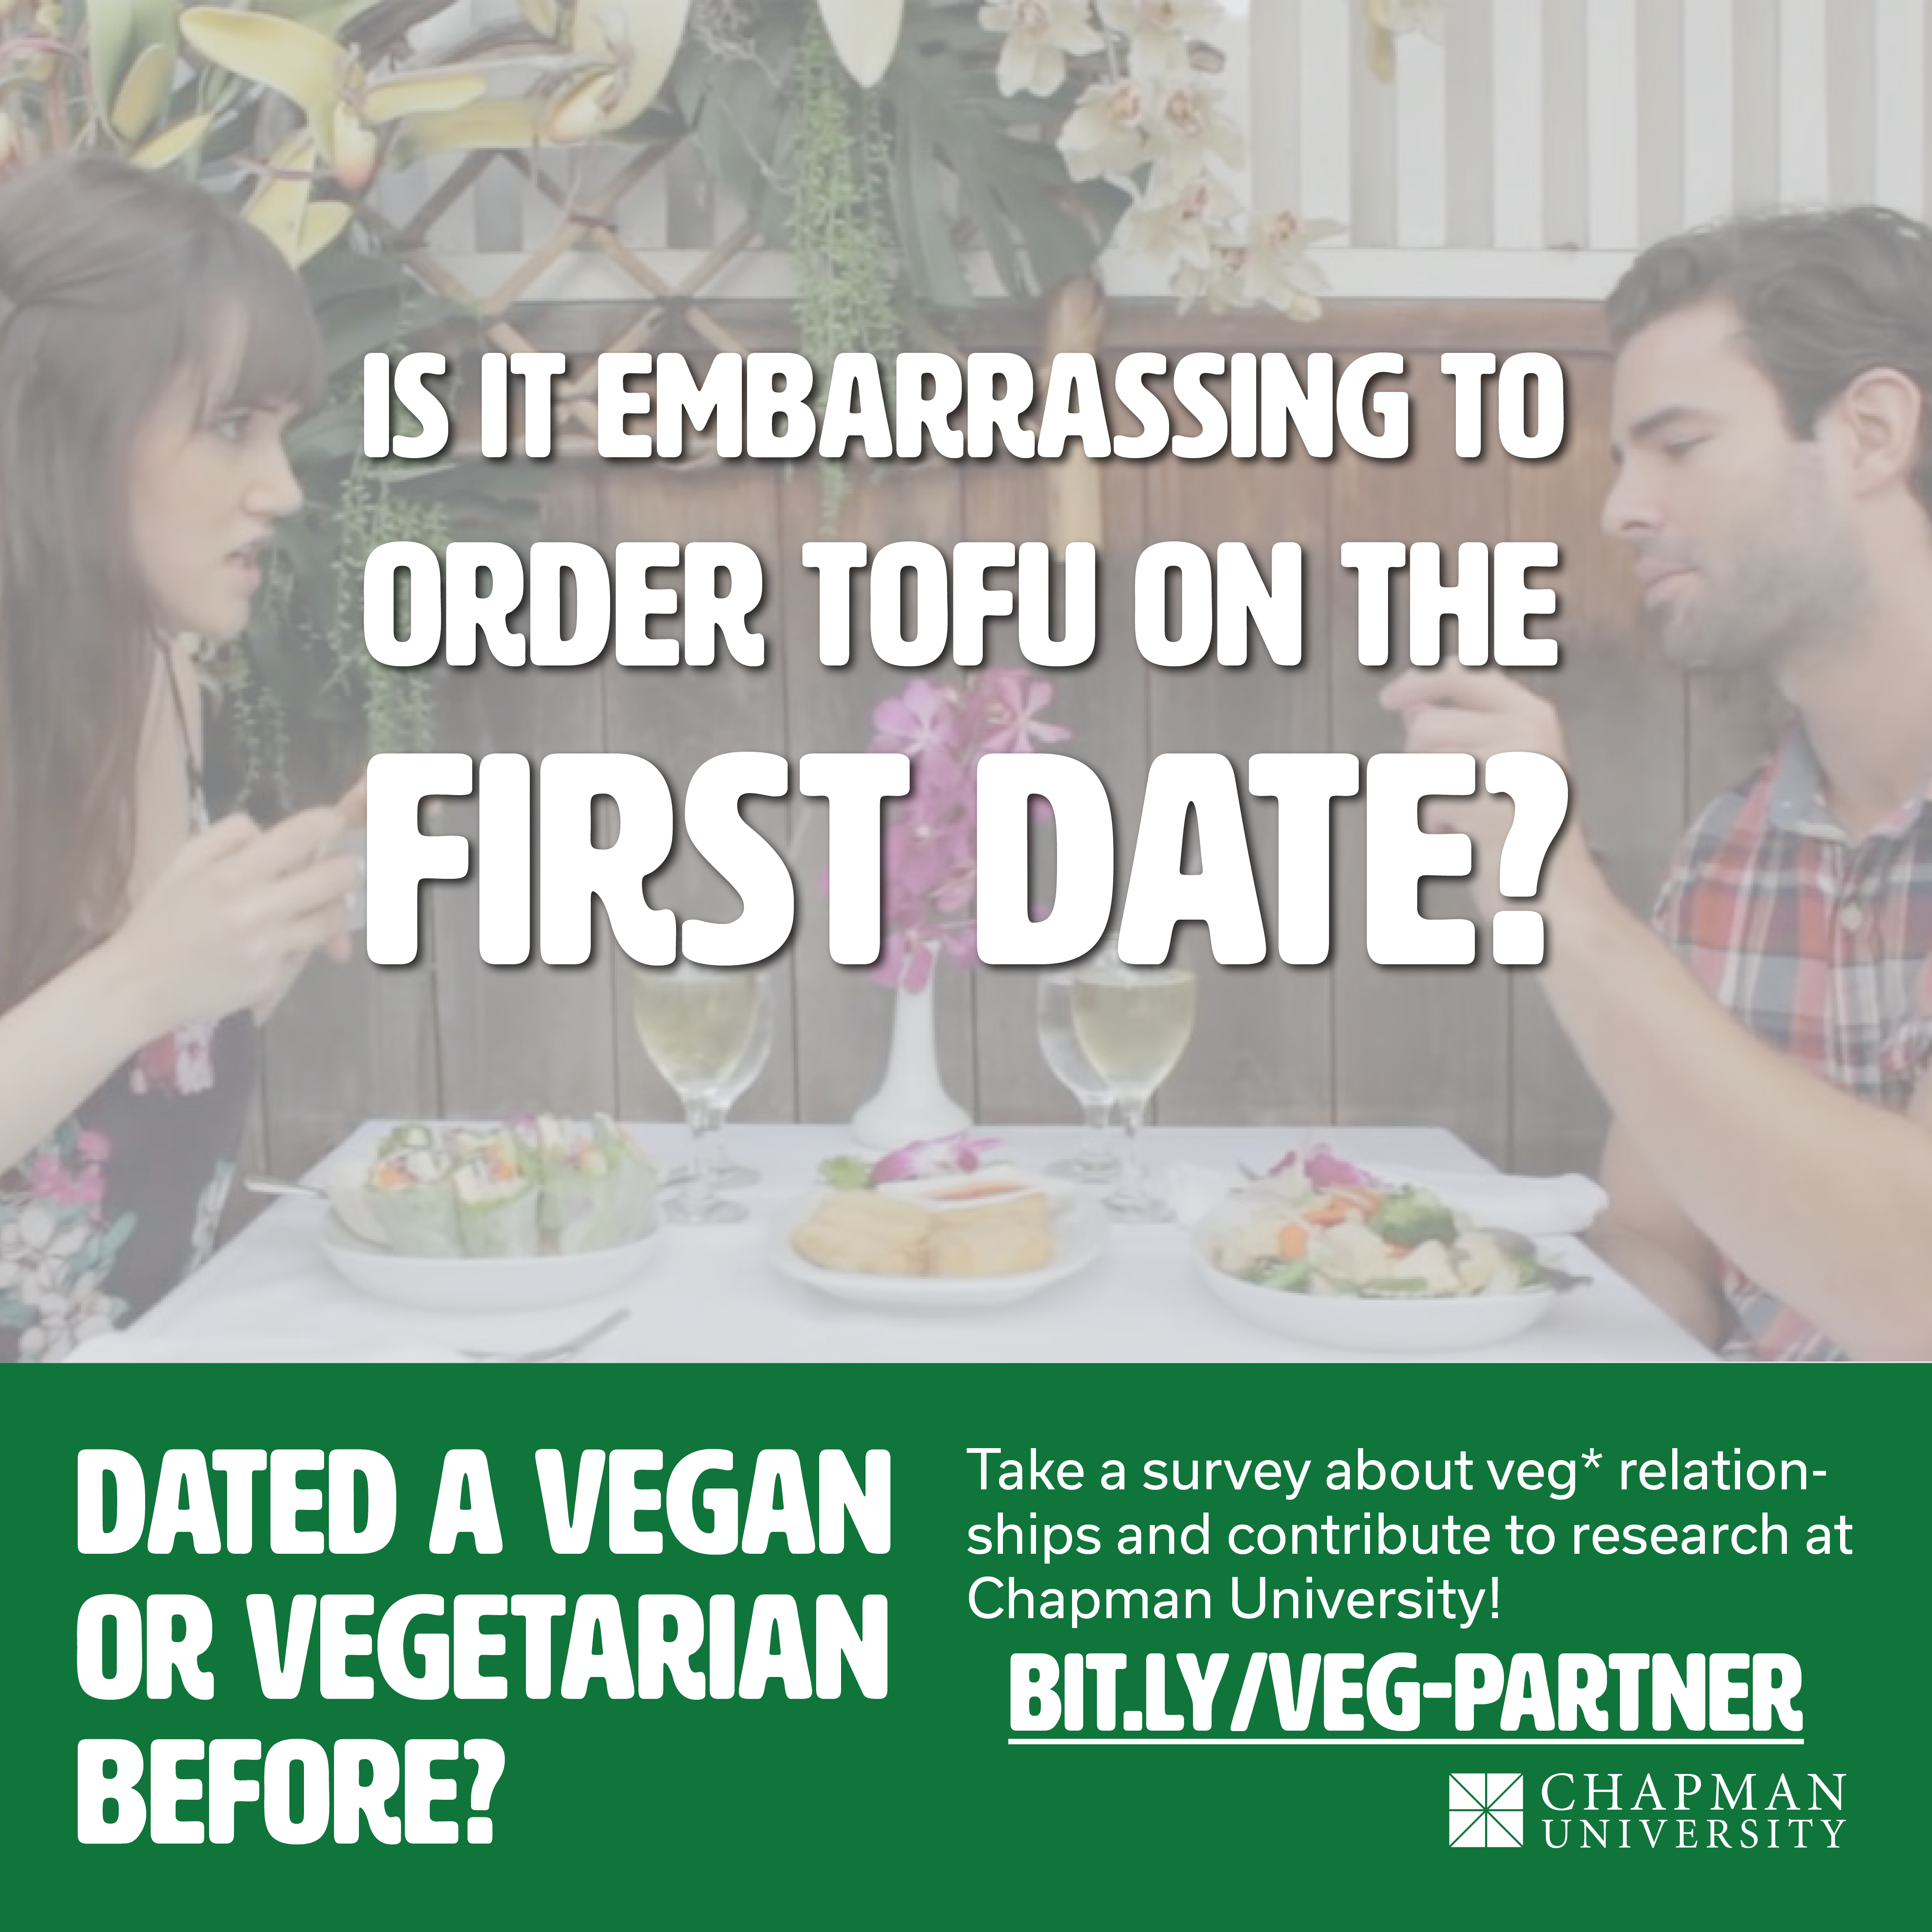
\includegraphics[width=6.5in,height=6.5in]{images/soyboys.jpg}

\end{document}